%!TEX root = Main.tex
\documentclass[Main]{subfiles}

\begin{document}
\section{Localization} % (fold)
	\label{sec:localization}
In the first lesson, the problem of localization is covered. 
Localization is defined as “The ability for a machine to locate itself in an environment". 
GPS is a solution to this problem that is often used when precision is not essential, but for navigation inside a house, GPS is not precise enough. 
Therefore alternative sensors like a LIDAR or an ultrasonic sensor can be used. 
These sensors only provides raw data, so localization is necessary to convert the raw sensor data and prior knowledge about the environment, that is navigated in, into estimates of the most likely current location of a robot.

Two primary steps in a localization problem are introduced; Motion and Sensing.
To improve the estimate of the robots position, sensing is performed. 
When sensing, raw data from a sensor is obtained, and compared with a map of the current environment to estimate the most likely current position of the robot. 
This is done by using Bayes rule:
\begin{equation}
\label{eq:bayes_rule}
P(X_{xy}|Z) = \frac{P(Z|X_{xy})\cdot P(X_{xy})}{P(Z)} = \frac{P(Z|X_{xy})\cdot P(X_{xy})}{\sum_{x} \sum_{y} P(Z|X_{xy})\cdot P(X_{xy})}
\end{equation}
Here, $P(X_{xy})$ is the prior probability of the gridcell, $X_{xy}$, before the measurement, $Z$.
$P(X_{xy}|Z)$ is the posterior probability after the measurement. 
$P(Z|X_{xy})$ is the probability of the measurement belonging to the specific gridcell and $P(Z)$ is a normalization factor, which can also be calculated by $\sum_{x} \sum_{y} P(Z|X_{xy})\cdot P(X_{xy})$.

Motion is what happens when the robot moves. 
This adds uncertainty to the current estimate of the robots position, as there might be errors associated with moving. 
When turning, for example, a robot might turn 91\degree instead of 90\degree. 
Therefore, moving a robot makes its position more uncertain, as there is a chance of over- or undershooting a movement.

The concept of localization is best explained with an example, shown in \autoref{fig:WallE}.
These figures describes three cycles of localization. 
Notice how, between each figure, the previous posterior has become the new prior, with a movement and some uncertainty added. 
After the second movement and sensing, the robot is fairly certain it is located at the second door to the right, simply by using Bayes Theorem.\\
\begin{figure}[H]
	\centering
	\begin{subfigure}[b]{0.8\linewidth}
		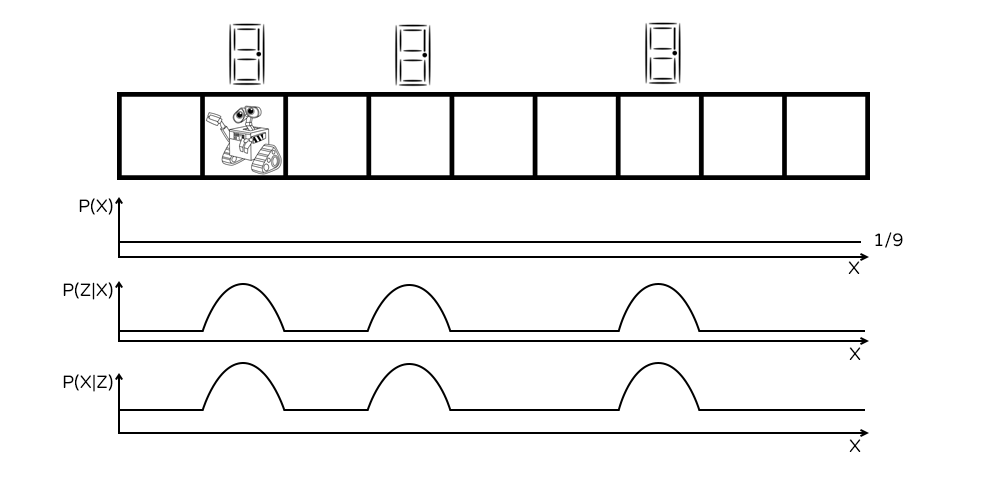
\includegraphics[width=\linewidth]{WallEOne}
		\caption{Initial sensing}
		\label{fig:WallEOne}
	\end{subfigure}\\
	\vspace{12pt} 
	\begin{subfigure}[b]{0.8\linewidth}
		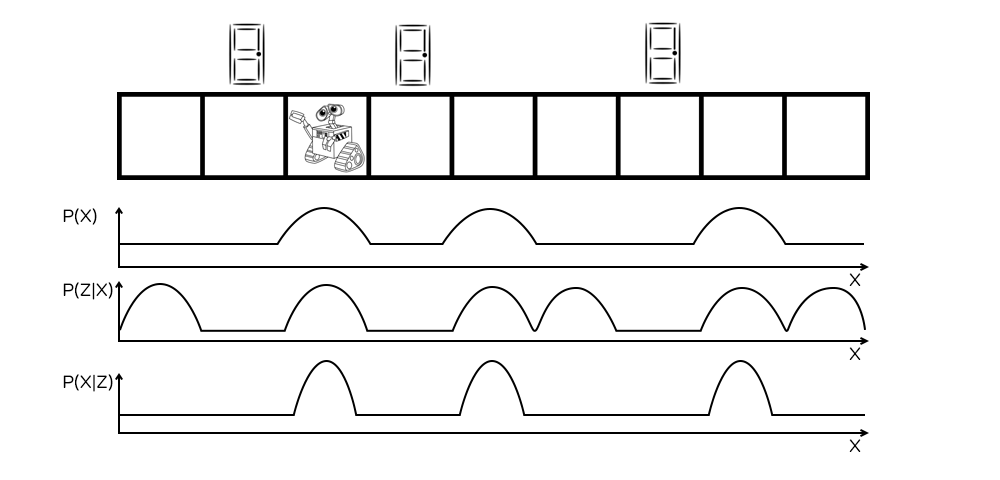
\includegraphics[width=\linewidth]{WallETwo}
		\caption{First move and second measurement}
		\label{fig:WallETwo}
	\end{subfigure}\\
	\vspace{12pt}
	\begin{subfigure}[b]{0.8\linewidth}
		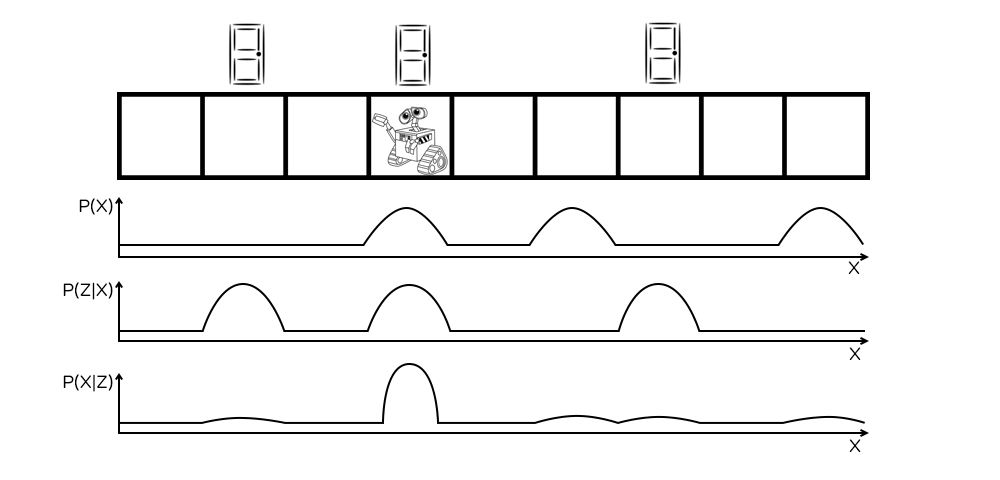
\includegraphics[width=\linewidth]{WallEThree}
		\caption{Second move and third measurement}
		\label{fig:WallEThree}
	\end{subfigure}
	\caption{Bayesian localization in three steps}
	\label{fig:WallE}
\end{figure}
\end{document}

